\chapter{建立你的 AI 科研绘图工作流}
\usetikzlibrary{decorations.pathreplacing}

环境科学专业的研究生小林正在撰写一篇关于农业流域河流硝态氮季节变化的论文。论文的第二张图（Figure 2）需要同时交代两件事：一是研究区“农田—地下排水管—支沟—河道—下游监测站”的物质传输路径；二是该站 2016 年全年的每日硝酸盐浓度与河流流量变化。导师看了一眼初稿大纲，只留下一句话：“把一年的监测数据和研究区画成一张图，让人一眼看出浓度跟流量的关系。”

小林立刻打开绘图工具，把从美国地质调查局（USGS）下载的日均值表格传了上去，输入一句：“帮我把这份河流数据画成一张专业的论文图，突出硝酸盐污染问题。”几十秒后，屏幕上出现了一张色彩鲜明、线条饱满的图表（后文图~\ref{fig:ch01-03} 将复现这类典型结果）。初看之下，这张图似乎可以直接放进论文；但准备写图注时，问题接连浮现：左右两条纵轴分别用红绿两色画在同一张图里，曲线交叉处让人误以为浓度与流量“数值相等”；9 月中旬原本有两天仪器缺测，图上却被一条直线直接连了过去；硝酸盐纵轴只写了“mg/L”，没写是按氮原子（以 N 计）还是按硝酸根离子（$\text{NO}_3^-$）计量；10 mg/L 处被画上一条醒目的红线并标着“超标！”，可那其实是针对市政处理后饮用水的标准，并不直接适用于未经处理的河水原水。

接着，她又用一句英文提示词生成研究区示意图（后文图~\ref{fig:ch01-05}）。生成的画面看起来像教科书插图，里面却多出了水处理厂建筑、大片绿色藻华，以及一整套“藻类死亡分解导致溶解氧下降”的生态机制图解——而她的论文既没有测溶解氧，也没有调查水厂。

一句模糊的指令，让工具替作者做出了十几个未经授权的科学决定。本章先解决这个根本问题：在动手输入提示词或运行脚本之前，先把制作科研图片的工作流程建立起来。

\section{给图片一个可以检验的任务}

一张科研图在论文中只承担一个核心任务。这个任务可以是“交代水样从农田进入河道的空间路径”，可以是“展示两个变量在一年十二个月里的同步起伏”，也可以是“比较同一批样本在处理前后的个体变化”。无论具体内容是什么，目标的表述都必须具体到能够直接约束图型、布局和标签。

“展示 2016 年的监测结果”之所以不合格，是因为它无法排除任何错误做法：把 366 天的数据求一个全年均值画成一根柱子，也叫“展示监测结果”；把缺测日悄悄插值补齐、把单位写漏，同样满足“展示监测结果”。相反，如果把任务写成可检验的句子，图的设计边界就立刻清晰起来。

在动笔或打开软件之前，先确定目标读者与核心信息，是科研可视化的基本准则。Rougier 等人（2014）在总结科研作图的十条规则时，把“了解你的读者”和“明确你要传递的信息”排在最前面。本书把这两条规则转化为每一张图开工前必须填写的一句话模板：

\begin{BookNote}
看完这张图，读者应该能够理解\_\_\_\_\_\_\_\_，并能从图中找到\_\_\_\_\_\_\_\_。
\end{BookNote}

前半句规定图片的表达目的，即读者读图后应当建立的整体认识；后半句规定读者可以在画面上逐一指认、核查的具体要素。目标句不需要预先迎合某种“漂亮结论”，相反，它要求图片如实容纳观测到的全部事实。

以小林的河流监测图为例，如果她把这句话写成：

\begin{BookNote}
看完这张图，读者应该能够理解 2016 年 Raccoon River 硝酸盐浓度的季节变化及其与河流流量在时间上的同步关系，并能从图中找到每日均值、缺测日、10 mg/L（以 N 计）参考线以及冬季流量的估算值时段。
\end{BookNote}

单凭这一句话，整张数据图的骨架就已经确定了大半：
\begin{itemize}
\item \textbf{决定图型：}要求读者找到“每日均值”和“缺测日”，意味着不能把数据汇总成月均柱状图或箱线图，必须保留按日排列的时间序列折线，并在缺测日处如实断开，不做平滑滤波或线性插值。
\item \textbf{决定布局：}要求理解浓度与流量“在时间上的同步关系”，同时两者物理量纲完全不同（浓度为 mg/L，流量为 $\text{m}^3/\text{s}$ 且跨越两个数量级），意味着最稳妥的布局是上下堆叠两个共享同一时间横轴的子图，让读者顺着垂直方向比对同一天的峰谷，而不是用容易产生视觉错觉的双 Y 轴把两条线叠在一起。
\item \textbf{决定标签与注释：}句中明确写出“10 mg/L（以 N 计）参考线”和“估算值时段”，直接提醒作者纵轴单位必须标明“以 N 计”，参考线旁必须注明“饮用水标准，仅作参照”，冬季受冰期影响的流量估算值必须在视觉上与实测值区分开来。
\end{itemize}

同样的道理也适用于其他研究设计。例如，当手头是一组样本在实验前后的配对测量值时，如果目标句写的是“理解每个对象在两次测量中的前后变化方向是否一致，并能从图中找到全部对象的配对观测值与逆向变化个体”，那么只画均值和标准差的柱状图就会直接出局，保留个体连线的配对点线图才符合要求（Weissgerber 等，2015）。第 2 章与第 5 章将专门拿这类配对数据拆解从任务定义到统计图表制作的全过程。

当你发现自己很难填完上面那句话的后半格——说不清读者到底应该在图上看到哪些具体元素——通常说明研究思路本身还没有理顺。先停下来把这句话改到可核查，比在绘图工具里盲目尝试二十次提示词更省时间。第 2 章将详细讨论如何把这一句话扩展为完整的绘图任务书。

\section{先判断自己正在处理什么}

写好目标句之后，第二步是清点手头的原始材料。本书从实际操作出发，把制作科研图的材料分成三大类：数值与数据表、解释性内容（文字、草图与已确认的关系）、仪器或现场获取的图像。这是一种面向工具选择与核验责任的操作分类，同一篇论文乃至同一张组合图里，经常同时包含这三类材料。

\begin{center}\footnotesize
\setlength{\tabcolsep}{3pt}
\renewcommand{\arraystretch}{1.15}
\begin{tabularx}{\linewidth}{@{}>{\raggedright\arraybackslash}p{24mm}>{\raggedright\arraybackslash}p{26mm}YY@{}}
\toprule
\textbf{材料类别} & \textbf{图片主要表达什么} & \textbf{本案例对应物与工具路线} & \textbf{作者必须核对什么} \\
\midrule
数值和数据表 & 数量、分布、时间变化与变量关系 & USGS 05484500 站 2016 年日均硝酸盐与流量表；走确定性绘图脚本或 \scidraw{} 科学可视化（\sdtool{sci-vis}）生成面板 b & 原始数值、计量单位、缺测日断开、质量码标记、坐标变换与统计含义 \\
文字、草图与已确认的关系 & 空间结构、实验方法、机制路径与概念解释 & 流域农田地下排水汇入河道及下游监测站位置的文献与站点描述；走 \scidraw{} 生成底图加人工叠字，形成面板 a & 对象增删、数量、水流或作用方向、边界条件，以及是否画出了未支持的污染源或机制 \\
仪器或现场获取的图像 & 实际观测到的形态、条带、显微信号或现场空间信息 & （若研究包含）现场传感器安装照片或遥感影像；保留原始图像，走图像呈现与组图流程（本案例未使用） & 未改动的原始文件备份、比例尺校准、通道与裁切记录、批次可比性，严禁生成式美化 \\
\bottomrule
\end{tabularx}
\end{center}

为什么要先做这道分类题？因为不同材料在论文里承担的\textbf{证据功能}截然不同，对应的制作工具和禁用操作也完全不同（图~\ref{fig:ch01-02}）。

\begin{figure}[htbp]\centering
\resizebox{\linewidth}{!}{\providecommand{\route}[1]{{\scriptsize\color{BookTeal}#1}}
\providecommand{\authcheck}[1]{{\scriptsize\color{BookInk!75}#1}}
\begin{tikzpicture}[
  card/.style={draw=BookTeal,fill=BookPale,rounded corners=2pt,text width=39mm,align=center,font=\small,minimum height=62mm},
  cardunused/.style={card,dashed,draw=gray,text=BookInk!80},
  icon/.style={font=\footnotesize},
  route/.style={font=\scriptsize,text=BookTeal},
  check/.style={font=\scriptsize,text=BookInk!75},
  bracebox/.style={draw=BookInk,rounded corners=1pt,font=\small,inner sep=3pt}
]
\node[card] (d) at (0,0) {%
  \begin{tikzpicture}[scale=0.55,baseline=(t.base)]
    \foreach \x in {0,1,2} {
      \foreach \y in {0,1,2} {
        \draw[BookInk!60] (\x*0.35,\y*0.28) rectangle ++(0.32,0.24);
      }
    }
    \coordinate (t) at (0.35,0.5);
  \end{tikzpicture}\\[2mm]
  数据\\[1mm]
  USGS 日均值\\（硝酸盐、流量）\\[2mm]
  {\route 确定性绘图 / 科学可视化 → 面板 b}\\[2mm]
  {\authcheck 作者核对：原值、单位、缺测、质量码}};
\node[card,right=7mm of d] (i) {%
  \begin{tikzpicture}[scale=0.55,baseline=(c.base)]
    \foreach \x/\n in {0/1,1/2,2/3} {
      \fill[BookTeal!40] (\x*0.55,0.15) circle (0.07);
      \node at (\x*0.55,0.15) {\tiny\n};
    }
    \draw[-{Stealth},BookInk] (0.07,0.15)--(0.43,0.15);
    \draw[-{Stealth},BookInk] (0.62,0.15)--(0.98,0.15);
    \coordinate (c) at (0.55,0.15);
  \end{tikzpicture}\\[2mm]
  解释性内容\\[1mm]
  研究区与排水路径的文字描述\\[2mm]
  {\route 生成绘图 → 面板 a}\\[2mm]
  {\authcheck 作者核对：对象、方向、是否画出未支持的来源}};
\node[cardunused,right=7mm of i] (p) {%
  \begin{tikzpicture}[scale=0.55,baseline=(cam.base)]
    \draw[BookInk!70,rounded corners=1pt] (0,0.05) rectangle (0.55,0.38);
    \draw[BookInk!70] (0.55,0.28)--(0.72,0.38)--(0.72,0.05)--(0.55,0.05);
    \fill[BookInk!50] (0.22,0.21) circle (0.09);
    \coordinate (cam) at (0.28,0.21);
  \end{tikzpicture}\\[2mm]
  现场/仪器图像\\[1mm]
  （如有）传感器或采样点照片\\[2mm]
  {\route 原图呈现与组图 → 本案例未使用}\\[2mm]
  {\authcheck 作者核对：原始文件、处理记录}};
\node[font=\scriptsize,text=BookInk!70,anchor=north] at ($(p.south)+(0,-2mm)$) {本例未使用};
\draw[BookInk!50,thick,decorate,decoration={brace,mirror,amplitude=4pt}] ($(d.south west)+(0,-6mm)$) -- ($(p.south east)+(0,-6mm)$);
\node[bracebox,below=9mm of i] (fig) {Figure 2（a \textbar\ b）};
\draw[BookInk!60] (i.south) -- ++(0,-5mm) -| (fig.north);
\draw[BookInk!60] (d.south) -- ++(0,-5mm) -| (fig.north);
\end{tikzpicture}
}
\caption{本章 Figure 2 用到的材料类别。面板 b 是证据，来自数据，走确定性绘图；面板 a 是解释，来自已确认的文字描述，走生成绘图。实验或现场图像属于第三类，本例未使用，第 8 章专门讨论。}\label{fig:ch01-02}
\end{figure}

第一类材料是\textbf{数值和数据表}。数据图在论文中是直接支撑结论的经验性证据。图中每一个点的横纵坐标都必须严格对应数据表里的真实记录，任何平滑、插值、剔除异常值或坐标轴非线性变换（如对数刻度）都直接影响读者的定量判断。因此，数据图必须走确定性绘图路线——无论是编写 Python/R 脚本，还是使用 \scidraw{} 的科学可视化模块（\sdtool{sci-vis}）读取表格并执行绘图代码。绝对不能把数据表或期望的曲线形状塞进纯文生图的图像生成模型里，让模型去“画”一条看起来像折线图的位图；图像生成模型不懂数值映射，它画出的波峰和波谷只是像素拼贴，不是你的观测数据。第 5 章将系统讲解数据图的制作与核验。

第二类材料是\textbf{文字、草图与已确认的关系}。当你需要向读者解释研究区的空间结构、实验步骤的先后顺序或分子生物学中的信号通路时，你手里拿的是文字描述或铅笔草图。由这类材料制作的方法流程图（第 6 章）和机制示意图（第 7 章），其功能是帮助读者理解背景与研究框架，本身不直接充当定量测量证据。在这里，图像生成工具（如 \scidraw{} 的 \sdtool{ai-drawing}、\sdtool{workflow-diagram-generator} 或 \sdtool{mechanism-figure-generator}）可以发挥很大作用：它能根据你的结构描述或草图快速生成构图候选与无文字视觉底图。但解释性图件有一条铁律：\textbf{示意图只能画出你手头材料与文献明确支持的对象和关系，不能“顺手”添加未经证实的因果链条。}在小林的案例中，面板 a 的任务只是交代“农田—地下排水管—支沟—河流—监测站”的监测背景；如果生成模型在河边多画了一座排污工厂或水处理厂，或者在水下画了富营养化耗氧过程，读者就会把右侧面板 b 里的硝酸盐浓度波动归因于那些虚构出来的设施或生态过程。

第三类材料是\textbf{仪器或现场获取的图像}，例如显微镜照片、蛋白印迹（Western blot）、病理切片、电镜图或野外采样点实拍照片。它们和数值表一样，属于原始观测证据。对这类材料，合规的操作仅限于在不改变像素证据的前提下做规范裁剪、对齐、添加校准比例尺、标注通道名称和排版组图（第 8 章）；绝不能把模糊的电泳条带或荧光图像丢进生成式模型里做“超分辨率重绘”或“去噪美化”，那在学术出版规范中属于篡改原始图像。

搞清这三类材料的边界后，面对任何复杂的组合图或图形摘要（第 10 章），你都可以先把它拆成单个面板：哪个面板是数据证据，哪个面板是概念解释，哪个面板是原始影像，各自走各自的制作通道，最后再回到组图工具里合成为一张整图。

\section{把工作分成六个环节}

许多研究生在画论文配图时之所以反复返工，是因为把所有事情混在了一个动作里：一边在对话框里改提示词，一边临时查数据单位，一边猜导师想要什么版式，改了十几轮之后连哪一版对应哪个数据文件都分不清了。

要让作图过程可控，不需要搭建繁琐的软件工程体系，只需把一张图的生命周期固定为六个环节：\textbf{说明任务、准备材料、制作初稿、检查并修改、组织说明、检查与交付}（图~\ref{fig:ch01-01}）。

\begin{figure}[htbp]\centering
\resizebox{\linewidth}{!}{\begin{tikzpicture}[
  box/.style={draw=BookTeal,rounded corners=2pt,fill=BookPale,minimum width=34mm,minimum height=12mm,align=center,font=\small},
  link/.style={-{Stealth[length=2mm]},thick,draw=BookInk},
  loop/.style={-{Stealth[length=1.8mm]},dashed,draw=BookInk!60},
  note/.style={font=\scriptsize,text=BookInk!70,align=center}
]
\node[box] (a) {说明任务};
\node[box,right=9mm of a] (b) {准备材料};
\node[box,right=9mm of b] (c) {制作初稿};
\node[box,below=18mm of c] (d) {检查并修改};
\node[box,left=9mm of d] (e) {组织说明};
\node[box,left=9mm of e] (f) {检查与交付};
\node[note,below=5mm of a] {任务书 v1};
\node[note,below=5mm of b] {数据字典};
\node[note,below=5mm of c] {d1、s1};
\node[note,below=5mm of d] {修改单};
\node[note,below=5mm of e] {组图与图注};
\node[note,below=5mm of f] {交付包};
\draw[link] (a)--(b);
\draw[link] (b)--(c);
\draw[link] (c)--(d);
\draw[link] (d)--(e);
\draw[link] (e)--(f);
\draw[loop] (d.north west) to[bend right=42] (b.south);
\draw[loop] (f.north) to[bend right=48] (a.south);
\node[note,align=center,text width=18mm] at ($(b.south)!0.45!(d.north west)+(0,-10mm)$) {发现问题时返回};
\node[note,align=center,text width=18mm] at ($(a.south)!0.45!(f.north)+(-22mm,2mm)$) {发现问题时返回};
\end{tikzpicture}
}
\caption{本书的六个环节。不适用的环节可以省略；核查发现问题时，返回产生问题的环节，而不是在当前环节反复重画。灰色小字为本章河流硝酸盐案例在各环节留下的产物（其中 d1、s1 分别代表数据面板初稿与示意面板初稿）。}\label{fig:ch01-01}
\end{figure}

这六个环节并不是一条只能硬着头皮往前走的单行道。正如图~\ref{fig:ch01-01} 中两条虚线回路所示，当你在“检查并修改”或“检查与交付”环节发现问题时，最关键的动作是\textbf{判断这个问题究竟产生于哪一个上游环节，然后退回那个环节去修}，而不是停留在当前环节盲目重画。下面逐一说明每个环节的核心工作，以及 AI、确定性工具与作者各自的分工。

\textbf{第一环节：说明任务。}在打开任何生成页面之前，先写清这张图的用途（哪篇论文的第几张图、单栏还是双栏尺寸）、目标读者、那句可检验的目标句、必须包含的对象与关系、视觉与排版约束，以及明确的禁用项和验收条件。AI 可以根据你的初步描述协助梳理栏目并提醒缺项；作者则负责决定研究问题、区分已知事实与假设、敲定验收标准。任务书的写法将在第 2 章展开；草图推演与视觉语言规范将分别在第 3 章和第 4 章展开。

\textbf{第二环节：准备材料。}把作图所需的原始数据表、站点元数据、文献依据或原始实验图像收集到同一个源文件夹中，检查版本一致性，编写简明的数据字典或材料说明。AI 可以协助编写下载与解析脚本、扫描空值与质量码、起草字段说明表；作者必须对照官方参数手册核实物理量单位（如区分“以 N 计”与“以 $\text{NO}_3^-$ 计”），确认采用已审定数据而非临时数据，并锁定未改动的原始文件备份。

\textbf{第三环节：制作初稿。}根据第 1.2 节判定的材料类别，分别进入对应工具生成第一版候选图。数据面板走确定性绘图脚本或科学可视化模块（第 5 章），方法与机制示意走流程图或示意图生成模块（第 6、7 章），实验原图走规范裁剪与标注流程（第 8 章）。AI 与绘图工具负责按明确指令绘制图表或生成无文字示意底图；作者负责把任务书转化为提示词或脚本参数，原样保存每一次实际提交的输入文本，并对候选结果做初步筛选。

\textbf{第四环节：检查并修改。}拿着任务书和数据字典逐条核对初稿，先查科学事实与数据准确性，再查构图、配色与字号，把发现的问题列成结构化的修改单。AI 负责执行具体修改指令；作者负责诊断错误根源并决定退回路径——若发现单位写错或空值被当成 0 读入，应沿图~\ref{fig:ch01-01} 的回路退回“准备材料”修正解析逻辑；若发现把饮用水标准写成了河水“超标”，则应退回“说明任务”厘清概念边界。每次修改后作者都必须对新图做全量复核，尤其检查未要求改动的部分是否被意外改变。第 11 章将专门讲解从初稿到可用稿的分层修改策略。

\textbf{第五环节：组织说明。}多面板组合时，确定网格比例、阅读顺序和面板编号（a、b……），在底图上叠加准确的矢量标签，并编写与图面严格对应的图注。组图工具（\sdtool{multi-panel-figure-maker}）可完成网格排版、编号与尺寸预设，图注辅助工具（\sdtool{figure-legend}）可根据画面起草图注框架；作者则必须补齐画面之外的关键信息（站号、下载日期、换算系数、缺测与估算说明、参考线适用范围），并删去任何未经证实的推测。组图与图注见第 9 章，图形摘要与汇报海报见第 10 章和第 12 章。

\textbf{第六环节：检查与交付。}按目标期刊的实际印刷尺寸（如双栏宽 174 mm）100\% 缩放看图，检查最小字号、线宽、分辨率与色觉可读性，最后将源文件、任务书、草稿、终稿、图注和 AI 使用说明打包归档。图片检查工具（\sdtool{figure-checker}）可自动检测分辨率、色彩模式与对比度风险；作者则负责最终的科学内容核验与投稿合规自查。第 13 章将系统总结核验与交付规范。

\section{一张图从任务书到终稿：河流硝酸盐案例}

现在，我们跟着小林的农业流域河流硝酸盐课题，把上面六个环节完整走一遍。

研究对象位于美国艾奥瓦州中西部的 Raccoon River 流域，该流域以玉米—大豆轮作农田为主，农田下普遍铺设地下排水暗管（tile drainage）。前人对该流域的研究表明，降水与土壤水经地下排水管和基流进入河道，是流域硝态氮输出的主要途径（Schilling 与 Zhang，2004）；原位紫外硝酸盐传感器则使研究者能够以日分辨率连续追踪河水硝酸盐浓度随水文过程的变化（Pellerin 等，2016）。

小林从 USGS 国家水信息系统（NWIS）获取了下游 Van Meter 水文站（站号 05484500）2016 年全年的公开日均值数据。这里必须明确一条科学红线：\textbf{本图只展示 2016 年该站点硝酸盐浓度与河流流量在时间上的共同变化，以及从农田排水到监测站的基本空间关系；本图不作污染来源定量归因，不计算氮负荷，也不作因果推断或显著性检验。}图中引用的美国环保局（EPA）饮用水最大污染物浓度（MCL）10 mg/L（以 N 计），法定适用对象是处理后的公共饮用水，河水原水不适用“超标”表述，图中仅作数值参照。

\textbf{环节一：说明任务——写出可核验的任务书。}吸取了开篇失败尝试的教训，小林先把目标句扩写为一份结构化的绘图任务书，保存在自己课题文件夹的文本文件里，之后在 \scidraw{} 科研绘图向导（\sdtool{figure-workflow}）选定路线、进入各步工具时再把它粘贴进去。以下展示核心栏目，完整提示词见本书仓库（\texttt{cases/} 目录）：

\begin{Prompt}
【用途与读者】环境科学论文 Figure 2，双栏宽 174 mm、高约 110 mm；读者为水文与水质同行。
【目标】理解 2016 年 Raccoon River 硝酸盐浓度的季节变化及其与流量的时间同步关系，
并能从图中找到每日均值、缺测日、10 mg/L（以 N 计）参考线和冰期估算流量时段。
【材料】(1) USGS 05484500 站 2016 年已审定日均值（硝酸盐 mg/L 以 N 计；流量 ft³/s）；
(2) 流域农田与地下排水汇入河道的文献与站点描述（Schilling & Zhang 2004）。
【对象与关系】面板 a（左，约 36% 宽）：农田 → 地下排水管 → 支沟 → 河道 → 监测站；
面板 b（右，约 62% 宽）：上下两个共享月份横轴的子图（上为硝酸盐，下为流量，不画因果箭头）。
【视觉】白底；数据图每子图单色且色觉友好；示意图扁平二维、低饱和、底图禁含任何文字。
【限制】不平滑、不插值、不删观测值；缺测日断开；流量换算为 m³/s 并取对数刻度；
10 mg/L 线仅作参照，不写“超标”；示意图禁画未支持的工厂、排污口、死鱼或藻华。
【验收】363 个硝酸盐日值与 366 个流量日值齐备；3 处缺测断开；极值（5 月 13 日 13.9、
9 月 16 日 3.19）可核查；174 mm 宽印刷时所有文字 >= 6 pt。
\end{Prompt}

这份任务书把设计推演变成了严密的因果链：因为【目标】要求看清每日浓度与流量的同步起伏，而【材料】表明两者单位与量级不同，所以【对象与关系】直接定为“上下两个共享月份横轴的子图”，排除了双 Y 轴；因为【材料】只有单站监测数据与农田排水文献背景，所以【限制】明确禁止画出工厂、排污口或死鱼，并在【验收】里写下了具体的点数（363 与 366）和极值日期（5 月 13 日与 9 月 16 日）。

\textbf{环节二：准备材料——数据字典与三个常见陷阱。}进入第二环节，小林用脚本从 USGS NWIS 日值服务下载了 05484500 站 2016 年原始数据文件（参数码 \texttt{99133} 为原位硝酸盐加亚硝酸盐日均值，参数码 \texttt{00060} 为日均流量，统计码 \texttt{00003} 代表日均；公有领域，引用 DOI 为 \texttt{10.5066/F7P55KJN}），解析为标准 CSV 数据表（\texttt{raccoon-2016-daily.csv}）。先看其中几行关键记录：

\begin{Prompt}
date,nitrate_mgL_as_N,nitrate_qual,discharge_cfs,discharge_qual
2016-01-01,12.1,A,6610,A
2016-01-08,11.1,A,4990,A:e
2016-05-01,8.66,A,16300,A
2016-05-13,13.9,A,10200,A
2016-09-16,3.19,A,5500,A
2016-09-18,,,7110,A
2016-09-19,,,8180,A
2016-12-14,,,968,A:e
\end{Prompt}

同时，她在数据说明文档中整理了数据字典与全表核验值：

\begin{center}\footnotesize
\setlength{\tabcolsep}{3pt}
\renewcommand{\arraystretch}{1.15}
\begin{tabularx}{\linewidth}{@{}l>{\raggedright\arraybackslash}p{26mm}>{\raggedright\arraybackslash}p{28mm}Y@{}}
\toprule
\textbf{字段名} & \textbf{物理含义} & \textbf{单位与编码} & \textbf{2016 年全表核验值} \\
\midrule
\texttt{date} & 日历日期 & \texttt{YYYY-MM-DD} & 共 366 行（闰年） \\
\texttt{nitrate\_mgL\_as\_N} & 原位硝酸盐+亚硝酸盐日均值 & mg/L（以 N 计）；空值为缺测 & 有值 363 天；缺测 3 天（9 月 18—19 日、12 月 14 日）；最大 13.9（5 月 13 日），最小 3.19（9 月 16 日）；$>10\ \text{mg/L}$ 共 162 天；5 月月均最高（12.84），9 月最低（5.36），1 月亦达 11.75 \\
\texttt{nitrate\_qual} & 硝酸盐质量码 & \texttt{A} = 已审定 & 全部为 \texttt{A}，无临时数据 \\
\texttt{discharge\_cfs} & 河道日均流量 & $\text{ft}^3/\text{s}$；乘以 $0.028316846592$ 换算为 $\text{m}^3/\text{s}$ & 366 天全有值；最大 $16,300\ \text{ft}^3/\text{s}$（$\approx 461.6\ \text{m}^3/\text{s}$，5 月 1 日），最小 $411\ \text{ft}^3/\text{s}$（$\approx 11.6\ \text{m}^3/\text{s}$，9 月 6 日） \\
\texttt{discharge\_qual} & 流量质量码 & \texttt{A} = 已审定；\texttt{A:e} = 冰期估算值 & \texttt{A:e} 共 58 天，集中在 1—2 月与 12 月 \\
\bottomrule
\end{tabularx}
\end{center}

这份五列表格里藏着三个必须在数据准备阶段排雷的陷阱：

第一，\textbf{“以 N 计”与“以 $\text{NO}_3^-$ 计”相差 4.43 倍}。硝酸盐浓度既可按氮原子质量报告（mg/L as N，摩尔质量 $14.01\ \text{g/mol}$），也可按完整硝酸根离子报告（mg/L as $\text{NO}_3^-$，摩尔质量 $62.00\ \text{g/mol}$），同一水样后者是前者的 $62.00 / 14.01 \approx 4.43$ 倍。USGS 参数 \texttt{99133} 与美国 EPA 的 10 mg/L 标准均采用“以 N 计”。纵轴标签若漏写“以 N 计”，习惯按 $\text{NO}_3^-$ 读图的同行就会严重误判。

第二，\textbf{流量单位换算与量级跨度}。USGS 原始流量单位是 $\text{ft}^3/\text{s}$，而国际期刊通常使用 $\text{m}^3/\text{s}$。换算改变了图上全部读数（从 $411\text{--}16,300$ 变为 $11.6\text{--}461.6$），且极值相差近 40 倍，属于直接影响读图解释的变换，必须写进档案与图注。

第三，\textbf{缺测日与冰期估算值的保留}。2016 年有 3 天硝酸盐缺测，另有 58 天冬季流量受河冰影响被标为估算值（\texttt{A:e}）。若清洗数据时直接删除含空值的行，那三天的流量也会丢失，折线还会跨过缺测日直接连线；若忽略质量码列，读者就会把冰期估算值当成常规实测值。因此解析脚本必须保留全部 366 行、空值留空，并在作图时把 \texttt{A:e} 日期标出。

在这一环节，AI 可以帮写解析脚本、统计空值与质量码；但对照参数手册确认“以 N 计”、确认未混入临时数据并记录下载日期，必须由作者亲自完成。

\textbf{环节三：制作初稿——数据图的正反对比。}为了看清有无任务书约束的差别，先看只给一句模糊要求时的典型初稿：

\begin{Prompt}
帮我把这份河流数据画成一张专业的论文图，突出硝酸盐污染问题。
\end{Prompt}

缺乏明确的任务约束时，默认绘图脚本或自动可视化很容易生成类似图~\ref{fig:ch01-03} 的问题初稿。

\begin{figure}[htbp]\centering
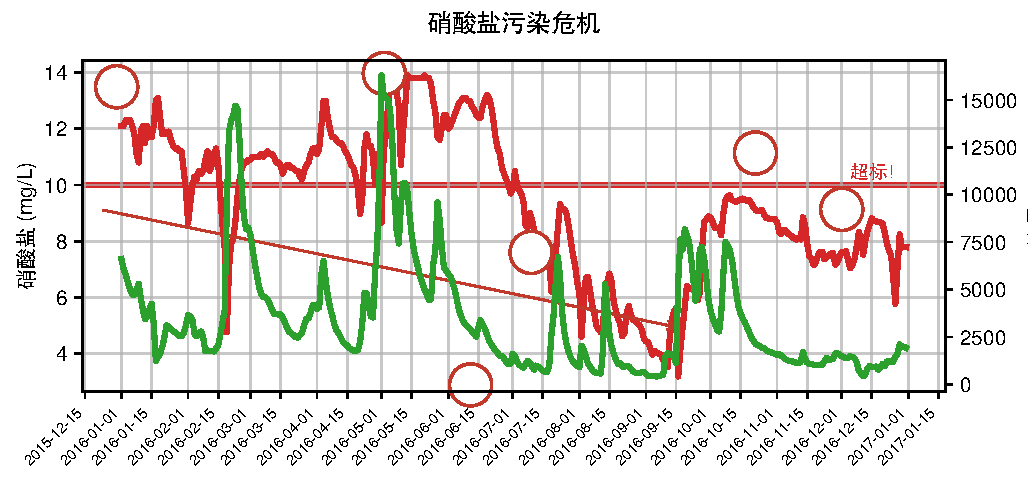
\includegraphics[width=\linewidth]{figures/ch01/ch01-03-nitrate-draft-vague-zh.pdf}
\caption{模糊要求下常见的数据图问题示例（基于真实 USGS 日均值构造的反例）。图中 (1) 双轴与红绿配色、(2) 跨过缺测日的连线、(3) 不完整的单位、(4) 把饮用水参照线写成“超标！”、(5) 带结论的标题、(6) 拥挤的日期刻度，都会让读者误读。}\label{fig:ch01-03}
\end{figure}

对照任务书检查这张初稿，图~\ref{fig:ch01-03} 上用红圈标出的六处硬伤非常清楚：(1) 采用红绿双 Y 轴且右轴未做单位换算，两条曲线的交叉位置随纵轴范围任意移动，极易造成“某日浓度与流量数值相当”的视觉假象，且红绿撞色对色觉障碍读者极不友好；(2) 细箭头所指的 9 月 18—19 日与 12 月 14 日缺测处被绘图函数默认用直线连过，相当于凭空伪造了三天的连续观测值；(3) 左轴漏写“以 N 计”，右轴既无单位也未区分冬季冰期估算值；(4) $y=10$ 处画了刺眼的红实线并标“超标！”，把市政饮用水标准错误套用到未经处理的河水原水上；(5) 顶部冠以“硝酸盐污染危机”的煽动性标题，越俎代庖替读者下结论；(6) 横轴按半月输出完整年月日字符串，字号拥挤越界，浓重的背景网格线反而喧宾夺主。

现在看按任务书约束的做法。在 \scidraw{} 科学可视化（\sdtool{sci-vis}）中上传 \texttt{raccoon-2016-daily.csv} 后，输入如下结构化指令：

\begin{Prompt}
读取上传的 raccoon-2016-daily.csv。date 为日期；nitrate_mgL_as_N 为
硝酸盐+亚硝酸盐日均值（mg/L，以 N 计）；discharge_cfs 为日均流量（ft³/s）。
绘制上下两个共享横轴的子图，不要使用双 Y 轴：
上图：硝酸盐日均值折线；纵轴“硝酸盐（mg/L，以 N 计）”；在 10 处画一条
灰色虚线，旁注“美国 EPA 饮用水 MCL 10 mg/L（以 N 计），仅作参照”。
下图：流量换算为 m³/s（乘以 0.028316846592），纵轴用对数刻度，
标“流量（m³/s，对数刻度）”；discharge_qual 为 A:e 的日期用浅色标出。
数值为空的日期在曲线上断开，不要插值、平滑或删除任何行。
横轴按月标注 2016 年 1–12 月。每个子图只用一种颜色，色觉友好。
不加标题，不加“超标”“污染”等结论性文字。
\end{Prompt}

按上述规则执行确定性绘图后，即可得到规范的数据图面板（图~\ref{fig:ch01-04}）。

\begin{figure}[htbp]\centering
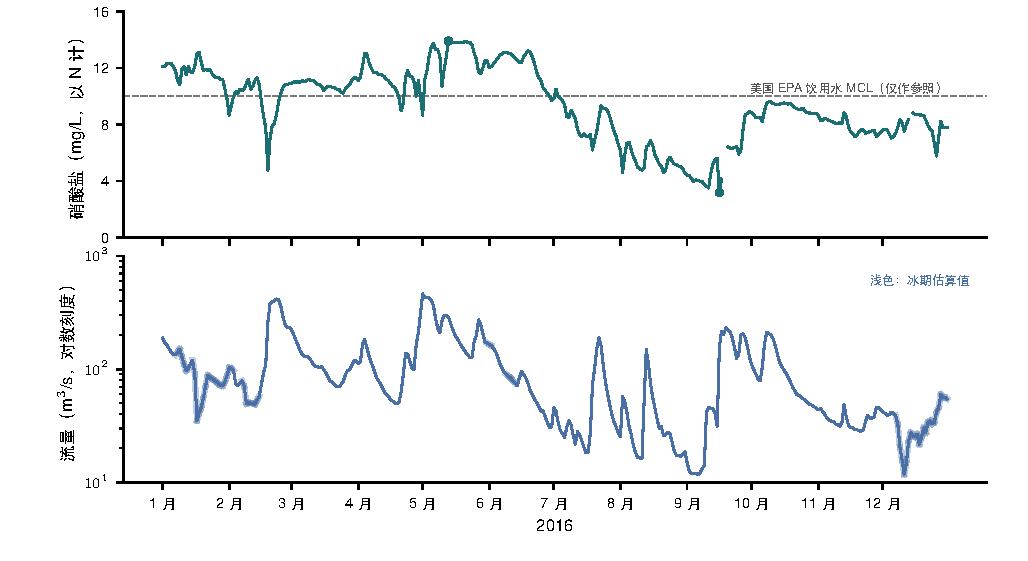
\includegraphics[width=\linewidth]{figures/ch01/ch01-04-nitrate-panel-brief-zh.pdf}
\caption{按任务书重绘的同一份数据。上：硝酸盐+亚硝酸盐日均浓度（mg/L，以 N 计），9 月 18—19 日与 12 月 14 日缺测处断开；灰色虚线为美国 EPA 饮用水最大污染物浓度 10 mg/L，仅作参照，河水原水不适用该标准。下：日均流量，由 $\text{ft}^3/\text{s}$ 换算为 $\text{m}^3/\text{s}$，对数刻度；浅色段为冰期估算值。数据：USGS 05484500，Raccoon River at Van Meter, IA，已审定日均值，2026 年 10 月 29 日下载。}\label{fig:ch01-04}
\end{figure}

对比图~\ref{fig:ch01-04} 与图~\ref{fig:ch01-03}，六处问题全部解决：上下子图共享月份横轴，既消除了双轴交叉错觉，又方便读者顺着垂直方向比对每次涨水过程与硝酸盐浓度的响应；上图在三个缺测日处如实留白断开，并用圆点标出 5 月 13 日全年峰值（13.9 mg/L）与 9 月 16 日谷值（3.19 mg/L）；$10\ \text{mg/L}$ 改为低调的灰色虚线并注明“仅作参照”；下图用对数刻度清晰展开跨越近两个数量级的流量变化，并用浅色宽线标出 58 天冰期估算值。从图上还能如实读出一个重要事实：2016 年虽然在 5 月出现最高月均浓度（12.84 mg/L）、9 月最低（5.36 mg/L），但 1 月份浓度同样处于高位（月均 11.75 mg/L）。只有拒绝平滑滤波与偏向性标题，才能让这些真实的季节特征完整呈现出来。

\textbf{环节三（续）：制作初稿——研究区示意图的正反对比。}接下来制作面板 a 的研究区示意图。同样先看只给一句模糊要求时会发生什么。如果向图像生成工具只输入一句宽泛的英文提示词：

\begin{Prompt}
Illustration of nitrate pollution in an agricultural river watershed. Aspect ratio 4:3.
\end{Prompt}

很多人以为模糊提示词的主要风险是生成扭曲的伪文字或冒烟的工厂烟囱。但我们把同一提示词连续生成了三次，结果给出了一个更值得警惕的教训：三次生成都没有出现工业烟囱或死鱼，图中的英文说明框和方向箭头也基本可读；然而模型为了诠释“污染（pollution）”，自作主张地塞进了大量\textbf{本案例材料根本没有支持的设施与生态机制}。图~\ref{fig:ch01-05} 是三次生成中的代表性结果，图中红圈 1—4 标出了画面中出现的四处问题。

\begin{figure}[htbp]\centering
\begin{tikzpicture}
\node[anchor=south west,inner sep=0] (img) at (0,0) {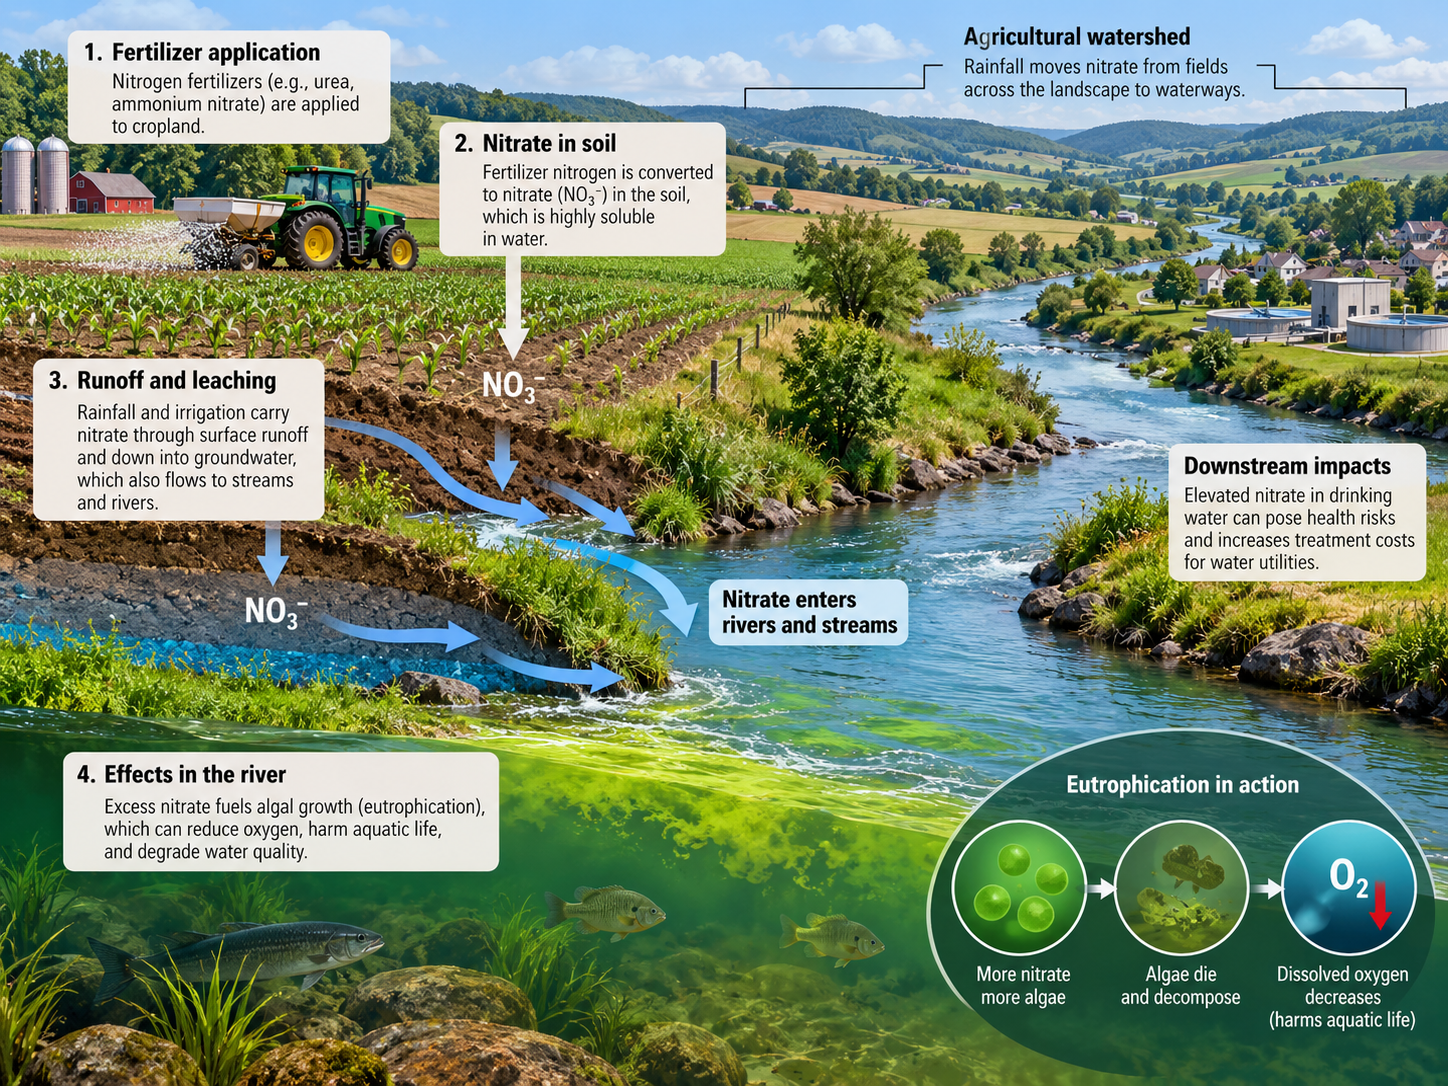
\includegraphics[width=\linewidth]{figures/ch01/ch01-05-site-schematic-vague.png}};
\begin{scope}[x={(img.south east)},y={(img.north west)}]
  \tikzset{badmark/.style={draw=red!80!black,very thick,circle,fill=white,fill opacity=0.88,text opacity=1,text=red!80!black,font=\bfseries\small,inner sep=1.2pt}}
  \node[badmark] at (0.88,0.72) {1};
  \node[badmark] at (0.80,0.22) {2};
  \node[badmark] at (0.22,0.80) {3};
  \node[badmark] at (0.62,0.45) {4};
\end{scope}
\end{tikzpicture}
\caption{用一句模糊要求生成的研究区示意图（本章示例图由图像模型生成，提示词与生成记录见本书仓库）。模型虽未生成工业排污烟囱或乱码，却加入了本案例材料并不支持的内容：(1) 右岸的水处理设施样建筑、聚落及饮用水处理成本说明，(2) 近景藻华、水下鱼群与右下角“富营养化—藻类分解—溶解氧下降”机制图解（同时漏掉了关键的农田地下排水管），(3) 写实风景、水下摄影透视与直接烧录在位图中的大段英文说明框，(4) 虽有径流箭头但缺少下游 USGS 监测站与传感器位置。}\label{fig:ch01-05}
\end{figure}

逐一核对这四处具体问题：
\begin{itemize}
\item \textbf{问题 (1)（未支持的水处理设施与成本说明）：}右岸（红圈 1）画出了聚落、带两个圆形池体的水处理设施样建筑，并配文讨论饮用水风险与水厂处理成本。本案例没有任何水厂位置或处理成本的数据，画入研究区面板会误导读者。
\item \textbf{问题 (2)（越界的富营养化机制与漏画排水管）：}近景与右下角（红圈 2）画出了大片绿色藻华、水下鱼群，以及“硝酸盐增加 $\rightarrow$ 藻类死亡分解 $\rightarrow$ 溶解氧（$\text{O}_2$）下降”的因果图解；而左侧土壤剖面只画了地表径流与地下水，反而漏掉了本流域最关键的农田地下排水管。把未测量的下游生态效应画成既定事实、同时漏掉核心传输通道，属于严重的科学失真。
\item \textbf{问题 (3)（写实装饰风格与锁死在位图中的文字）：}画面（红圈 3）采用写实天空、拖拉机远景与水下光影，且四个大段英文说明框直接烧录在位图里，字号、字体与语言均无法在后期单独修改。
\item \textbf{问题 (4)（缺少监测站位置）：}图中虽有径流箭头，但下游（红圈 4）没有标出 USGS 05484500 监测站与原位传感器，无法与面板 b 的数据建立空间对应。
\end{itemize}

要把示意图拉回正轨，核心是两条：一是明确列出\textbf{必须出现的科学对象}与\textbf{严格排除清单}；二是要求模型\textbf{只输出不含任何文字的干净底图}，文字标签留到后期在组图或矢量工具中单独叠加。修改后的结构化英文提示词关键部分如下（完整提示词见本书仓库 \texttt{cases/} 目录）：

\begin{Prompt}
Flat 2D scientific schematic for a journal figure panel, portrait 4:5, pure white
background. Clean vector style: flat fills, thin dark-gray outlines, no gradients,
no shadows, no 3D, no texture.
ABSOLUTELY NO TEXT: no letters, words, numbers, symbols, labels, legend, or title.
SCENE: simplified oblique (~30-degree) view of an agricultural landscape with a
cut-away soil block in the lower-left quarter.
- Upper half: 5-6 rectangular fields in muted sage green and wheat yellow; no buildings.
- Meandering river (soft blue) from upper-left to lower-right, joined by one tributary ditch.
- Lower-left soil cut-away: 3 round gray subsurface drain pipes, one outlet discharging
  into the tributary ditch.
- Lower-right river bank: simple gray monitoring station box with cable to a submerged
  cylindrical sensor; 2-3 hollow chevrons on water surface pointing downstream.
STRICTLY EXCLUDE: factories, chimneys, sewage pipes, towns, bridges, dead fish, algae,
murky water, warning signs, chemical symbols, clouds, decorative borders.
\end{Prompt}

即便提示词如此细致，生成结果仍需逐张核验筛选。我们把同一提示词生成了三次，结果各有差异：第 1 次生成中，左下角土壤剖面的受水沟与汇入主河道的支沟之间出现白色断口，“排水管 $\rightarrow$ 支沟 $\rightarrow$ 主河道”的水流路径被截断，因此淘汰；第 3 次生成画出了两条独立支沟分别汇入主河道，偏离了“单条支沟汇入”的设定，同样淘汰；只有第 2 次生成完整实现了白底、零文字、6 块农田、3 个灰色排水管口、连续汇入主河道的支沟、下游岸边的监测站与水下传感器，以及 3 个指向下游的白色 V 形流向标记，且排除清单中的干扰物均未出现。

把第 2 次生成图放大到 200\% 仔细核对，仍能看到四处细微偏差：支沟在入河前呈小 Y 形合流；右侧第三个排水管口直接兼作出水口；传感器停在水面波纹处而未完全画成深水浸没；土壤剖面与仪器箱体仍带轻微颗粒纹理和明暗过渡。由于这些细节不影响“农田—地下排水管—支沟—主河道—监测站”的核心空间拓扑，且画面干净无伪文字，可以在图注中注明“简化示意，不按比例”，再在预留的空白处叠加六个中文矢量标签，得到合格的研究区示意面板（图~\ref{fig:ch01-06}）。

\begin{figure}[htbp]\centering
\begin{tikzpicture}
\node[anchor=south west,inner sep=0] (img) at (0,0) {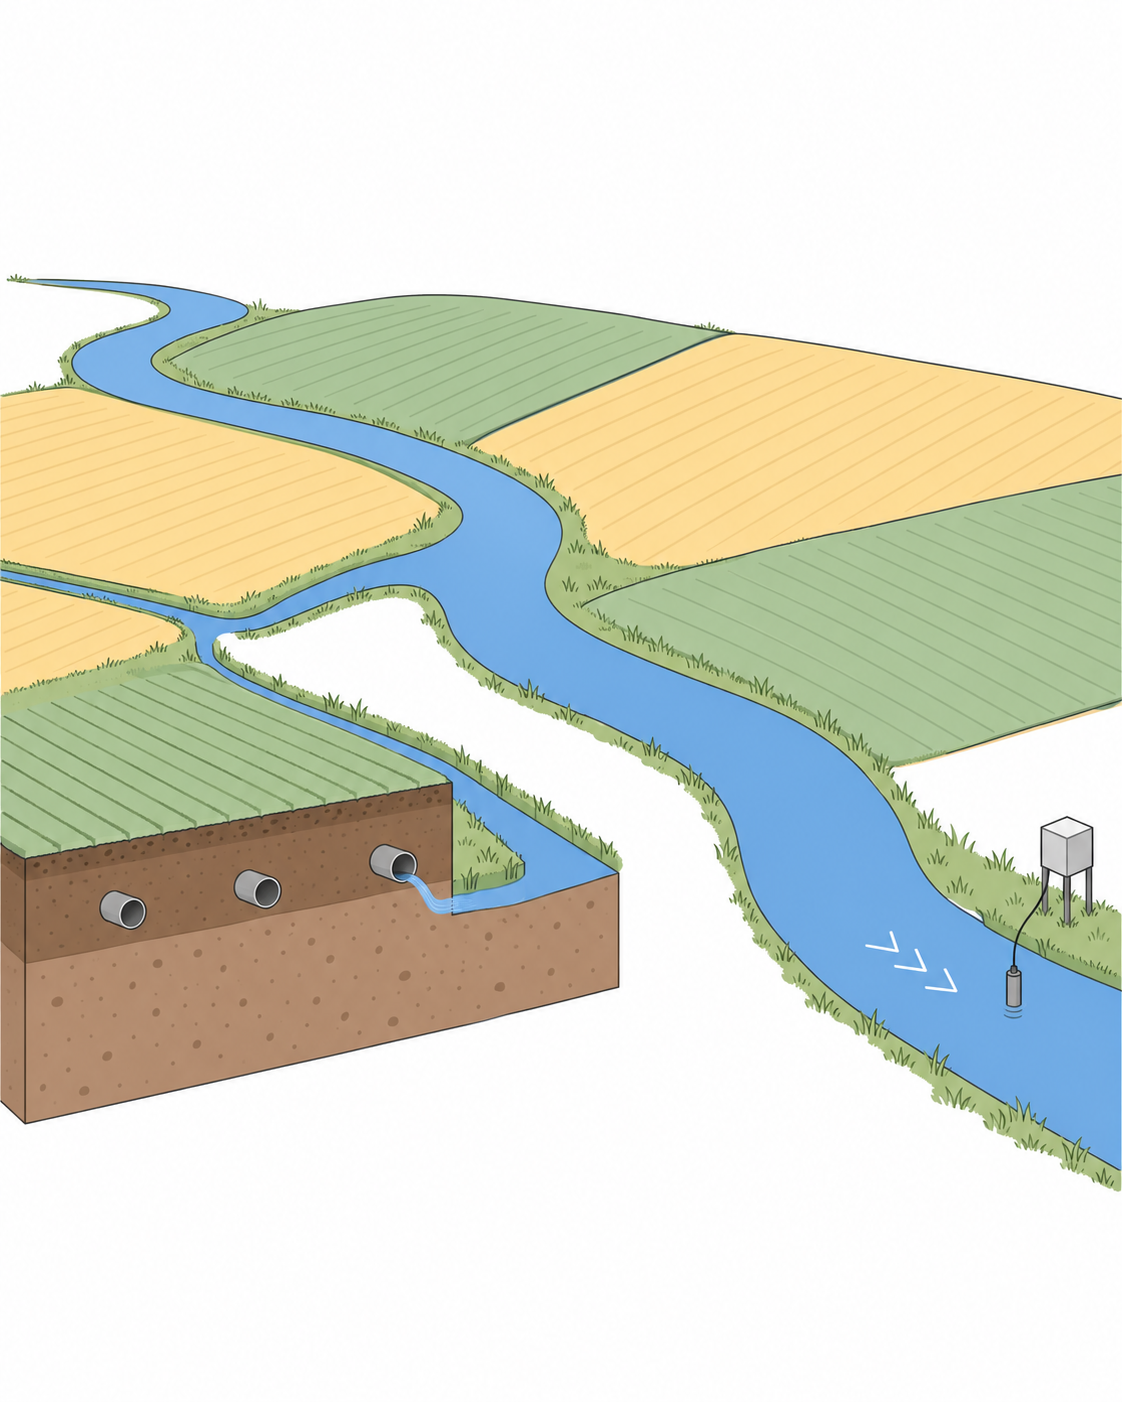
\includegraphics[width=0.62\linewidth]{figures/ch01/ch01-06-site-schematic-brief.png}};
\begin{scope}[x={(img.south east)},y={(img.north west)}]
  \tikzset{lbl/.style={font=\footnotesize,fill=white,fill opacity=0.82,text opacity=1,inner sep=1.5pt,align=center}}
  \node[lbl] at (0.50,0.88) {农田（玉米—大豆，示意）};
  \node[lbl] at (0.22,0.18) {地下排水管};
  \node[lbl] at (0.12,0.45) {支沟};
  \node[lbl] at (0.55,0.55) {Raccoon River};
  \node[lbl] at (0.80,0.12) {监测站 USGS 05484500};
  \node[lbl] at (0.72,0.36) {水流方向};
\end{scope}
\end{tikzpicture}
\caption{按任务书生成的研究区示意底图（三次生成中的第 2 次结果）及后期叠加的中文标签。底图不含任何生成文字，排除了无关设施与未证实的生态后果，清晰交代“农田—地下排水管—支沟—主河道—下游监测站”的空间关系。}\label{fig:ch01-06}
\end{figure}

\textbf{环节四：检查并修改——用修改单管理迭代。}面对初稿中的问题，不能只说“再改得专业一点”，而应将数据图初稿（图~\ref{fig:ch01-03}）与示意图初稿（图~\ref{fig:ch01-05}）的问题逐条对照任务书列成\textbf{修改单}，明确具体修改指令及退回环节：

\begin{center}\footnotesize
\setlength{\tabcolsep}{3pt}
\renewcommand{\arraystretch}{1.15}
\begin{tabularx}{\linewidth}{@{}c>{\raggedright\arraybackslash}p{32mm}>{\raggedright\arraybackslash}p{20mm}Y>{\raggedright\arraybackslash}p{22mm}@{}}
\toprule
\textbf{\#} & \textbf{初稿中发现的问题} & \textbf{违反的条款} & \textbf{可核查的修改指令} & \textbf{应退回的环节} \\
\midrule
1 & 双 Y 轴，两线交叉让人误以为“浓度与流量相等” & 【对象与关系】 & 拆为上下两个共享横轴的子图 & 制作初稿 \\
2 & 9 月 18—19 日与 12 月 14 日缺测被直线连过 & 【限制】【验收】 & 空值保留为 \texttt{NaN}，曲线在三处自然断开，不插值 & 准备材料（核查读入逻辑） \\
3 & 轴标签缺“以 N 计”；流量无单位且未换算 & 【材料】【限制】 & 写全单位；流量乘以 $0.028316846592$ 换算为 $\text{m}^3/\text{s}$ 并用对数轴 & 准备材料 \\
4 & $10\ \text{mg/L}$ 线标“超标！”；顶部带结论标题 & 【限制】 & 删标题；改为灰色虚线，标“饮用水 MCL（仅作参照）” & 说明任务（厘清解释边界） \\
5 & 红绿高饱和配色，半月全日期刻度拥挤越界 & 【视觉】 & 每子图一色、选色觉友好色；横轴改为 1—12 月刻度 & 制作初稿 \\
6 & 冬季 58 天冰期估算流量（\texttt{A:e}）与实测无区分 & 【目标】 & 用浅色宽线标出 \texttt{A:e} 日期，子图右上角加图例 & 制作初稿 \\
7 & 示意图初稿出现水处理厂、藻华与富营养化图解，漏掉地下排水管 & 【对象与关系】【限制】 & 不在原图上局部修补；按任务书对象与排除清单重新生成无文字底图 & 制作初稿 \\
8 & 示意图文字烧录在位图中，且第 1 次生成支沟断开、第 3 次两条支沟 & 【视觉】【对象与关系】 & 底图禁文字；核验选定路径连续的第 2 次生成底图，后期叠加矢量标签 & 检查并修改 \\
\bottomrule
\end{tabularx}
\end{center}

记住一条铁律：\textbf{每次修改后必须重新全量核验，包括原本没有要求改动的部分。}生成式重绘可能在修好支沟的同时弄丢监测站，脚本调整坐标轴间距也可能意外裁掉全年的峰值点。最稳妥的核验动作只有三个：一是把新旧两版图片并排叠放或快速切换，肉眼扫视未修改区域有无变形；二是拿数据字典里的极值日期与缺测日期直接在图上“按图索骥”，确认峰值、谷值与断点位置分毫不差；三是把画面放大到 200\% 逐一清点关键科学对象的数量与连接方向，把验收条款从头重勾一遍才算过关。

\textbf{环节五与环节六：组织说明、终尺寸检查与交付。}两个面板各自通过核验后，进入第五环节“组织说明”。在 \scidraw{} 中，可先将示意面板与数据面板下载到本地，再打开组图工具（\sdtool{multi-panel-figure-maker}），选择 $1 \times 2$ 网格、左 a 右 b 宽度比约 $36:62$、自动编号 \textbf{a}/\textbf{b}、期刊双栏宽 $174\ \text{mm}$ 预设，导出包含 TIFF、PNG、PDF、PPTX 与处理记录的 ZIP 包。将左右两个面板按预设网格对齐、统一留白与编号后，即合成为完整的论文 Figure 2（图~\ref{fig:ch01-07}）。

\begin{figure}[htbp]\centering
{\tikzset{text width/.code={}}\begin{tikzpicture}
\node[anchor=south west,inner sep=0] (panel) at (0,0) {%
  \begin{minipage}[t]{0.34\linewidth}
    \IfFileExists{figures/ch01/ch01-06-site-schematic-brief.png}{%
      \begin{tikzpicture}
      \node[anchor=south west,inner sep=0] (img) at (0,0) {%
        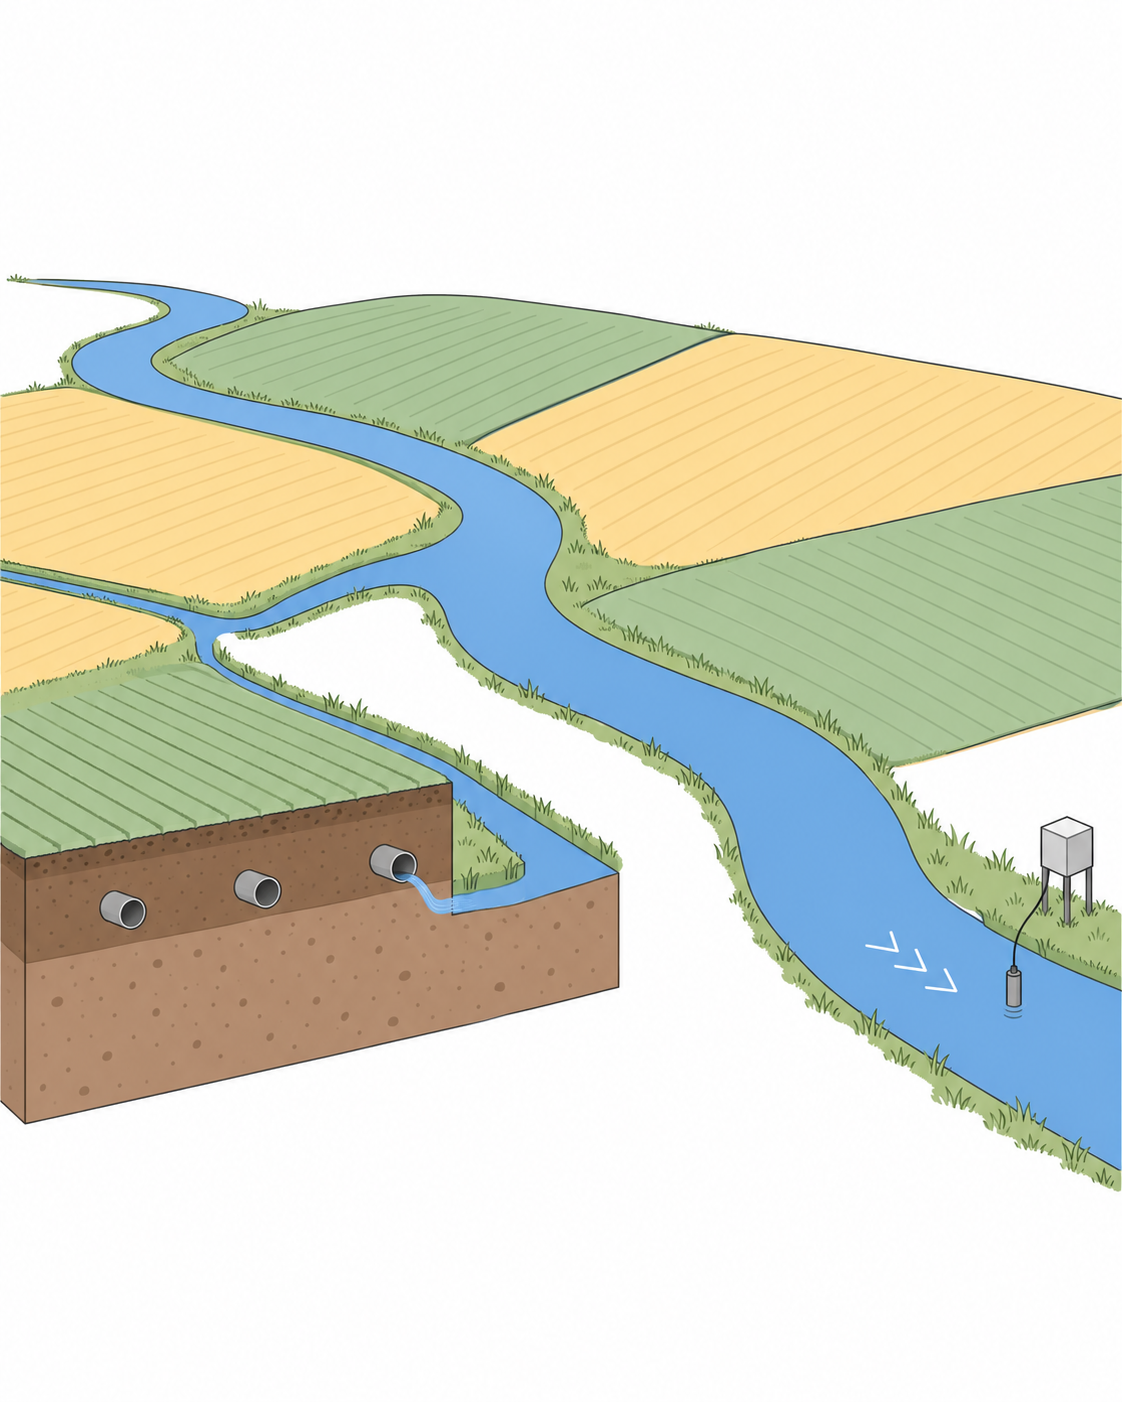
\includegraphics[width=\linewidth]{figures/ch01/ch01-06-site-schematic-brief.png}};
      \begin{scope}[x={(img.south east)},y={(img.north west)}]
        \tikzset{lbl/.style={font=\scriptsize,fill=white,fill opacity=0.8,text opacity=1,inner sep=1pt,align=center}}
        \node[lbl,text width=0.28,align=center] at (0.48,0.86) {农田（玉米—大豆，示意）};
        \node[lbl,text width=0.22,align=center] at (0.20,0.16) {地下排水管};
        \node[lbl,text width=0.18,align=center] at (0.10,0.44) {支沟};
        \node[lbl,text width=0.22,align=center] at (0.52,0.52) {Raccoon River};
        \node[lbl,text width=0.26,align=center] at (0.52,0.10) {监测站 USGS 05484500};
        \node[lbl] at (0.50,0.38) {水流方向};
      \end{scope}
      \end{tikzpicture}
    }{%
      \fbox{\parbox[c][0.36\linewidth][c]{0.34\linewidth}{\centering\scriptsize 缺少 ch01-06 底图\\（codex-image，未在本任务范围）}}
    }
    \par\vspace{1mm}{\scriptsize 示意，不按比例}
  \end{minipage}\hfill
  \begin{minipage}[t]{0.64\linewidth}
    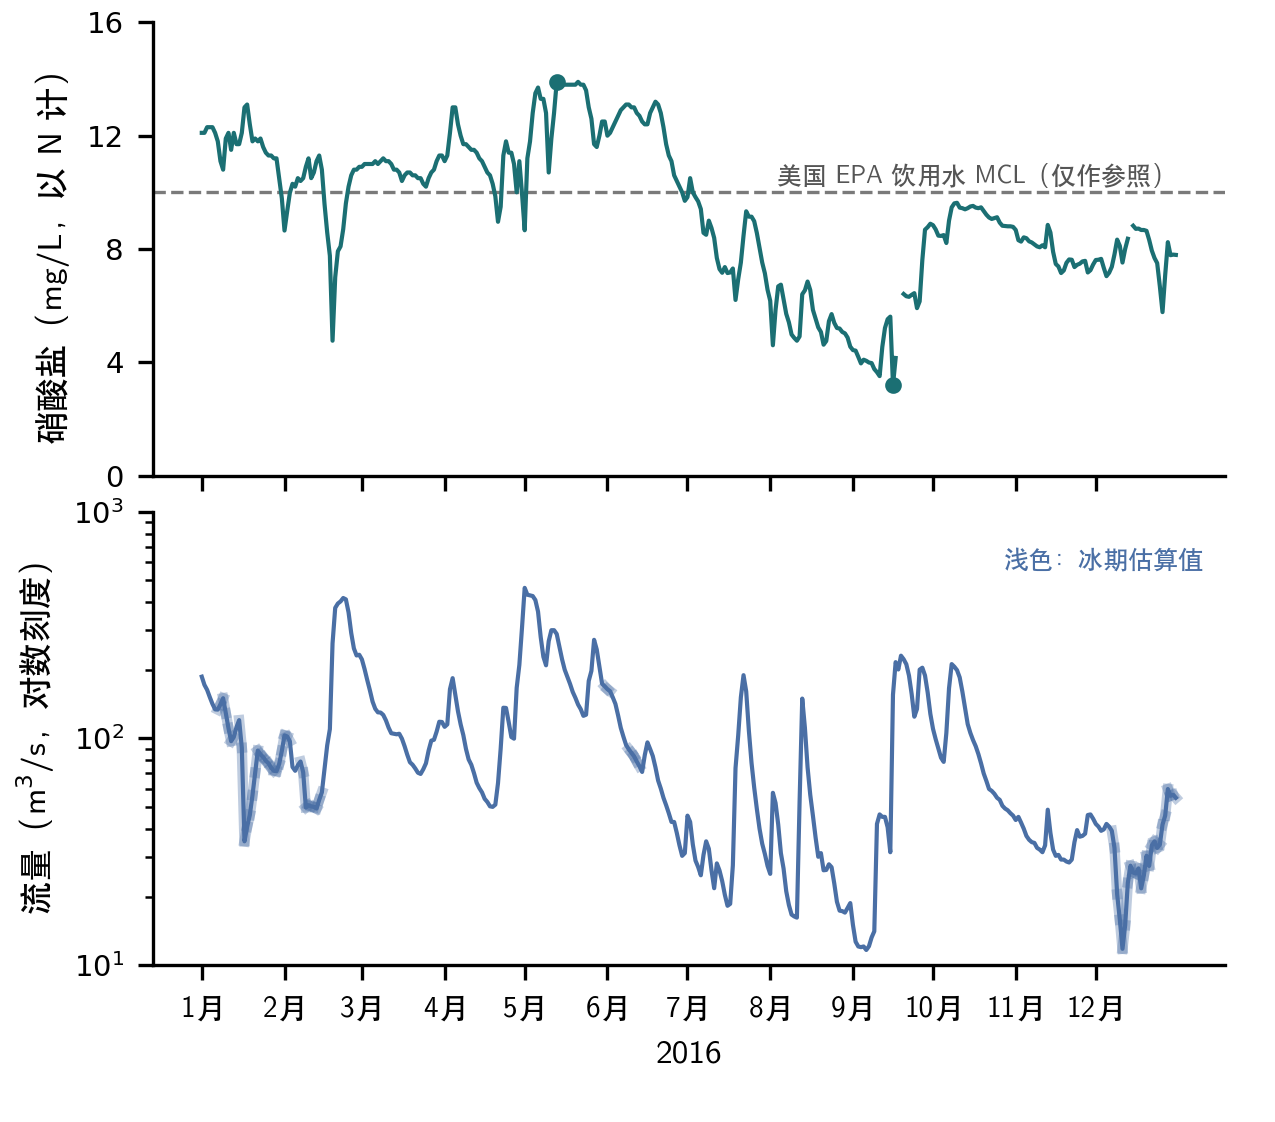
\includegraphics[width=\linewidth]{figures/ch01/ch01-04-nitrate-panel-brief-zh-panel.png}
  \end{minipage}};
\node[anchor=south west,font=\bfseries\small] at ([xshift=1mm,yshift=1mm]panel.north west) {a};
\node[anchor=south west,font=\bfseries\small] at ([xshift=0.34\linewidth,yshift=1mm]panel.north west) {b};
\end{tikzpicture}
}
\caption{\textbf{图 2 示例：2016 年 Raccoon River 的硝酸盐浓度与流量。}（a）研究区简化示意：农田地下排水经支沟汇入河道，下游为 USGS 监测站（05484500，Van Meter, IA）；不按比例，不表示具体地块、管网或污染来源。（b）上：硝酸盐+亚硝酸盐日均浓度（mg/L，以 N 计），缺测日断开；灰色虚线为美国 EPA 饮用水最大污染物浓度 10 mg/L（以 N 计），仅作参照。下：日均流量（$\text{m}^3/\text{s}$，由 $\text{ft}^3/\text{s}$ 换算，对数刻度），浅色段为冰期估算值。数据为 USGS 已审定日均值（公有领域），2026 年 10 月 29 日下载；本图不包含负荷计算或统计检验。示意底图由图像模型生成，标签由作者后期叠加；本章示例图的提示词与生成记录见本书仓库。}\label{fig:ch01-07}
\end{figure}

接着编写图注。若使用图注辅助工具（\sdtool{figure-legend}）上传终稿图起草初稿，作者必须清楚：\textbf{模型只能看到图面像素，不知道站号、下载日期、换算过程和法规适用边界。}作者必须亲手核对并补齐四件事：(1) 站点编号 05484500、地名、已审定状态与下载日期；(2) “以 N 计”单位、缺测断开、$\text{m}^3/\text{s}$ 对数刻度与冰期估算值说明；(3) 声明面板 a“不按比例，不表示具体地块、管网或污染来源”、$10\ \text{mg/L}$ 线“仅作参照”、且“不包含负荷计算或统计检验”（严禁编造样本量或统计量）；(4) 如实说明示意底图由生成工具制作、标签由作者添加。

最后进入第六环节“检查与交付”。先在 $174\ \text{mm}$ 实际印刷宽度下 100\% 缩放检查所有文字（均 $\ge 6\ \text{pt}$）与线条，确保叠加标签未遮挡排水管口或监测站图形；再用图片检查工具（\sdtool{figure-checker}）检测分辨率、色彩空间、灰度对比度与色觉风险。切记\textbf{技术检查通过不等于科学内容正确}，最后必须对照任务书【验收】条款逐项核查全部数据点、断点与图注表述，确认无误后打包归档。

\section{在 SciDraw AI 中选择路线}

打开 \scidraw{} 的“科研绘图向导”（\sdtool{figure-workflow}），先选择要做的图型：\textbf{机制图 / 流程图、数据图、多面板组图、图形摘要}（图~\ref{fig:ch01-08}）。选定后，页面给出一条 3–4 步的有序路线，每一步只有一句说明和一个打开对应工具的按钮。例如“机制图 / 流程图”路线依次为：生成初稿（机制图生成器；画流程图时改用流程图生成器）→ 修改细节（AI 绘图）→ 写图注（图注工具）→ 检查并导出（图片检查）。每一步都可以单独使用，已有初稿可直接从第 2 步开始。

\begin{figure}[htbp]\centering
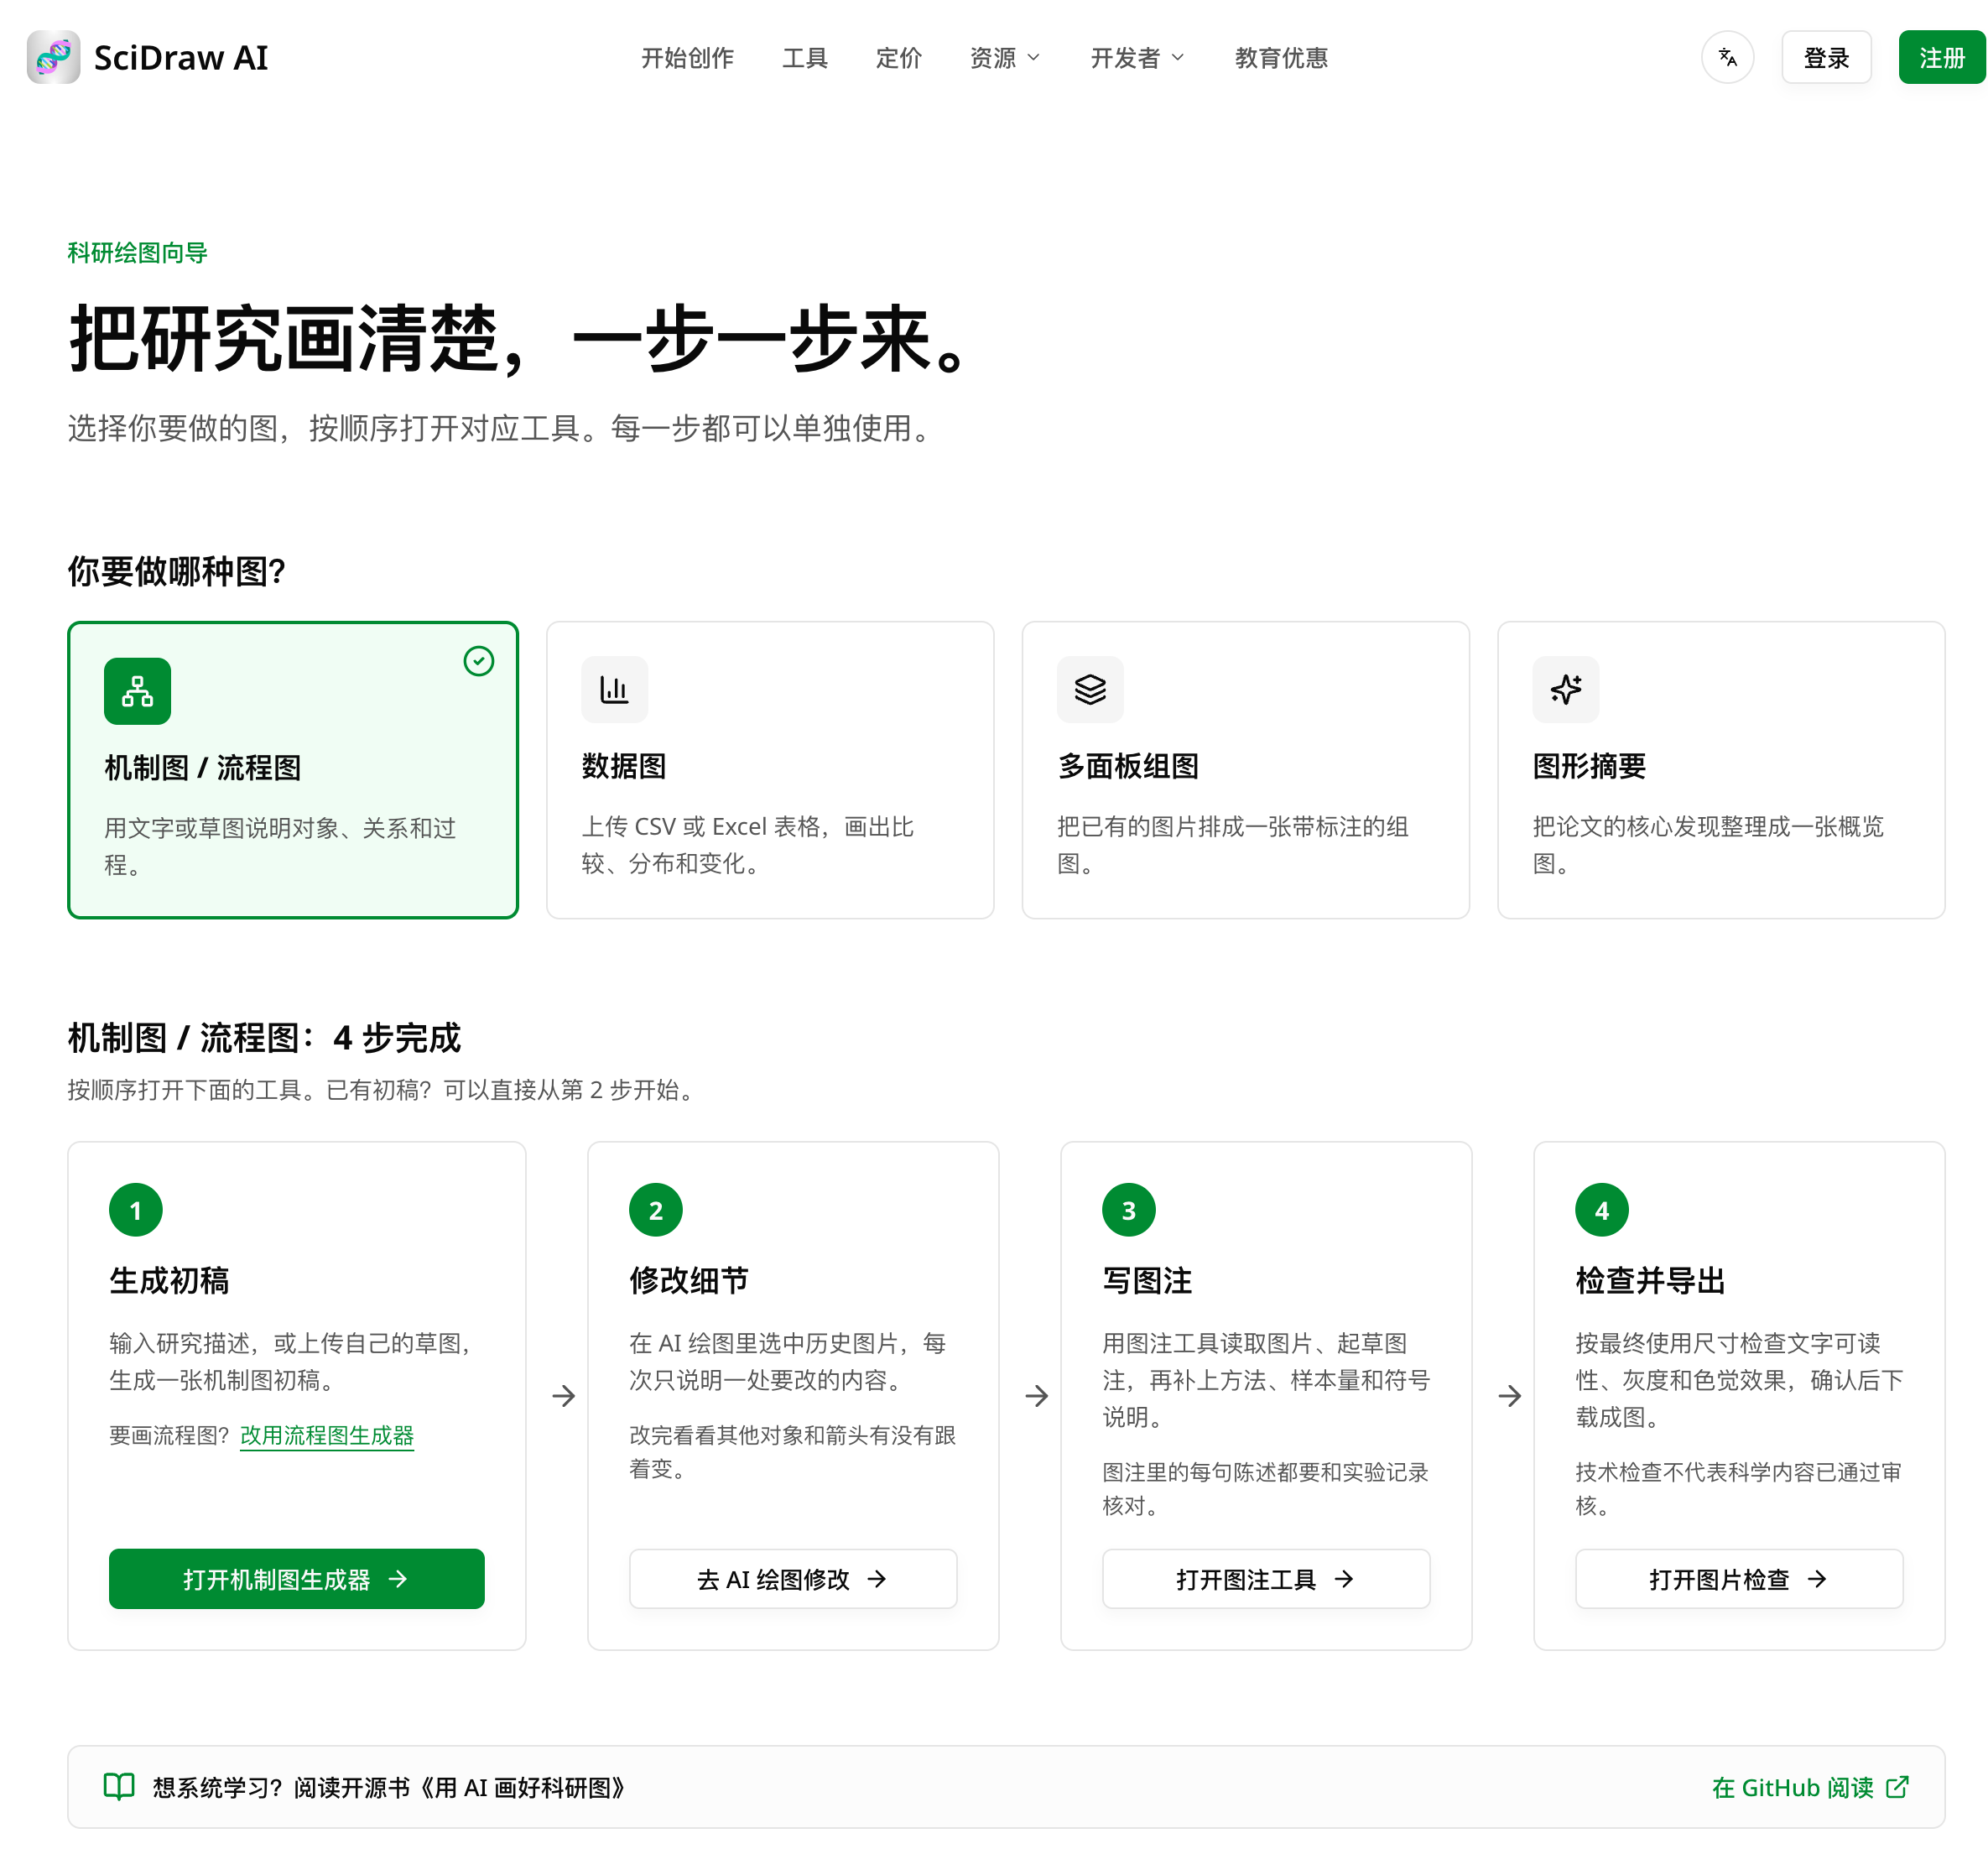
\includegraphics[width=0.92\linewidth,height=0.68\textheight,keepaspectratio]{figures/ch01/ch01-08-guide-ui-zh.png}
\caption{\scidraw{} 科研绘图向导（2026 年 10 月 30 日）。选中“机制图 / 流程图”后，页面列出四步路线——生成初稿、修改细节、写图注、检查并导出，每步附一句说明和打开对应工具的按钮。}\label{fig:ch01-08}
\end{figure}

一张组合图可以串联两条路线：本章案例先走“数据图”路线在科学可视化（\sdtool{sci-vis}）完成面板 b，再走“机制图 / 流程图”路线在流程图或绘图工具（\sdtool{workflow-diagram-generator}、\sdtool{ai-drawing}）完成面板 a，最后进入组图、图注和检查工具。如果你已有现成图片只需补写图注或检查分辨率，也可以直接点进对应步骤。

使用向导时需注意三项平台事实：
\begin{enumerate}
\item \textbf{向导不保存任务书和进度：}页面只给出路线和工具入口，没有任务书编辑框，也不记录你做到了哪一步。任务书写在自己的文档或文本文件里，存进课题文件夹作为记录，进入每一步的工具时粘贴进去。
\item \textbf{跨工具交接采用“下载—上传”：}向导的按钮只负责打开对应工具，不会自动传递任务书或图片；把单面板送往组图、图注或检查工具时，需先下载命名清楚的版本（如 \texttt{panel-b-nitrate-v2.pdf}）再上传，这也能防止误传旧草稿。
\item \textbf{向导不替你做科学审核：}它只给出步骤顺序和工具入口，核实单位、质量码与证据边界仍靠作者自己。
\end{enumerate}

\section{给每张图保留一个小型档案}

在本地硬盘或代码仓库中为每张图建一个结构固定的文件夹，几个月后审稿人要求补图或修改单位时就能随时复现。本章案例的小型档案结构如下：

\begin{Prompt}
fig2-raccoon-nitrate/
  source/   usgs-05484500-2016.rdb（原始下载备份，只读不改）
            raccoon-2016-daily.csv、data-dictionary.md（字段、单位、质量码、DOI、下载日期）
  brief/    figure2-brief-v1.txt（自己保存的任务书）、prompts-log.txt（实际提交的全部输入）
  drafts/   panel-b-draft1.pdf、panel-b-revised.pdf、panel-a-candidates/、
            revision-notes.md（初稿 8 项问题及回退修改记录）
  final/    figure2-final.pdf、figure2-final.tiff、legend-zh.txt、legend-en.txt、
            ai-use.md（使用的功能、日期、输入、采用输出、人工修改）、checks.md
  code/     fetch_usgs.py、plot_nitrate.py
\end{Prompt}

档案不必记录每次鼠标移动，但\textbf{凡是影响科学事实或定量解释的决定都必须留痕}：包括单位换算公式与坐标轴变换、缺测值与质量码的处理规则、示意图剔除无根据元素及从多次生成候选中择优的依据，以及参考线适用范围的界定。同时在 \texttt{ai-use.md} 中如实记录使用的工具功能、日期、实际输入、采用的输出及人工修改；正式投稿前应查阅目标期刊当时的 AI 使用与披露政策。

\section{AI 在这一步能做什么与不能做什么}

六个环节中 AI、确定性工具与作者的职责边界汇总于表~\ref{tab:ch01-01}。

\begin{table}[htbp]\centering\footnotesize
\setlength{\tabcolsep}{3pt}
\renewcommand{\arraystretch}{1.15}
\caption{六个作图环节中 AI 能做什么、不能做什么与作者必须核对的内容。}\label{tab:ch01-01}
\begin{tabularx}{\linewidth}{@{}>{\raggedright\arraybackslash}p{18mm}YYY@{}}
\toprule
\textbf{环节} & \textbf{AI 能做} & \textbf{AI 不能做} & \textbf{作者要核对} \\
\midrule
说明任务 & 根据你的描述起草任务书各栏；指出缺项（如单位、读者、尺寸） & 替你决定图要回答的研究问题；判断结论是否成立 & 目标句是否可检验；用途与尺寸是否真实 \\
准备材料 & 写下载/解析脚本；汇总缺测、质量码；起草数据字典 & 保证数据版本正确；判断“以 N 计”还是“以 $\text{NO}_3^-$ 计”而不读参数说明 & 单位、质量码、下载日期、是否混入临时数据 \\
制作初稿 & 数据图：按明确指令出图；示意图：快速给出构图候选 & 保证不插值、不平滑（除非你写明）；保证示意图不添加未支持的对象 & 逐条对照验收条件；数原始点数；查“多出来的东西” \\
检查并修改 & 执行具体修改指令；按问题表重出图 & 判断修改是否引入新错误；只改一处而不动其他部分（图像修改可能影响整张图） & 每次修改后重新全量核验，包括没要求改的部分 \\
组织说明 & 组图排版、编号、尺寸预设；起草图注 & 知道站号、下载日期、处理方式等图中看不见的信息；编造样本量和统计量是禁止的 & 图注每个数字与说明是否有出处 \\
检查与交付 & 技术检查（分辨率、色彩、灰度、色觉风险） & 科学审核；替你确认期刊 AI 政策 & 终尺寸可读性；交付包能否让他人复现 \\
\bottomrule
\end{tabularx}
\end{table}

\section{本章检查清单}

\begin{itemize}
\item 我能用一句话写出这张图的目标，并且它能决定图型、布局或标签。
\item 我已判断每个面板的材料类别，数据面板走确定性绘图，示意面板不画未经支持的对象。
\item 原始数据保留未改动的副本；单位、质量码、缺测与下载日期写进了数据说明。
\item 实际提交给工具的每段输入都保存了下来。
\item 每一版修改都有记录：改了什么、为什么、回到了哪个环节。
\item 终稿在实际使用尺寸下检查过文字和线条。
\item 图注中的每个数字、来源、处理方式都能在档案中找到依据。
\item 每一步的输出都是我对照任务书核对后才进入下一步的，而不是打开过工具页面就算完成。
\item 交付包里有 AI 使用记录；投稿前查过目标期刊当时的要求。
\end{itemize}

\section{练习}

\begin{enumerate}
\item \textbf{（目标句）}为本章案例另写两个不同的目标句：一个关注“春季高浓度持续多少天”，一个关注“低流量期的浓度”。分别说明它们会让图型、时间范围或标注怎样变化。
\item \textbf{（找错）}不看第 1.4 节修改单，列出图~\ref{fig:ch01-03} 与图~\ref{fig:ch01-05} 中至少 5 个问题，并为每个问题写一句可以核对的修改指令；再判断每个问题应回到六个环节中的哪一个。
\item \textbf{（\scidraw{} 实操）}从 USGS 下载另一个有硝酸盐传感器的站点（或你自己研究中的一份时间序列）的一年日均值，按第 1.4 节格式把任务书写在自己的文档里，再在科研绘图向导（\sdtool{figure-workflow}）选“数据图”，从第 1 步进入 \sdtool{sci-vis} 上传数据、粘贴任务书中的绘图要求，生成后对照验收条件逐条打勾，记录至少一次修改指令及其效果。把整个过程按第 1.6 节结构存档。
\end{enumerate}

\section*{参考文献}

\begin{itemize}
\item Pellerin BA, Stauffer BA, Young DA, Sullivan DJ, Bricker SB, Walbridge MR, Clyde GA, Shaw DM. Emerging tools for continuous nutrient monitoring networks: sensors advancing science and water resources protection. \textit{JAWRA Journal of the American Water Resources Association}. 2016;52(4):993--1008. doi:10.1111/1752-1688.12386
\item Rougier NP, Droettboom M, Bourne PE. Ten simple rules for better figures. \textit{PLoS Computational Biology}. 2014;10(9):e1003833. doi:10.1371/journal.pcbi.1003833
\item Schilling K, Zhang Y-K. Baseflow contribution to nitrate-nitrogen export from a large, agricultural watershed, USA. \textit{Journal of Hydrology}. 2004;295(1--4):305--316. doi:10.1016/j.jhydrol.2004.03.010
\item U.S. Environmental Protection Agency. National Primary Drinking Water Regulations (nitrate MCL 10 mg/L as N). \url{https://www.epa.gov/ground-water-and-drinking-water/national-primary-drinking-water-regulations}
\item U.S. Geological Survey. USGS water data for the Nation: National Water Information System database, site 05484500. \url{https://doi.org/10.5066/F7P55KJN} (accessed 2026-10-29).
\item Weissgerber TL, Milic NM, Winham SJ, Garovic VD. Beyond bar and line graphs: time for a new data presentation paradigm. \textit{PLOS Biology}. 2015;13(4):e1002128. doi:10.1371/journal.pbio.1002128
\end{itemize}
